\documentclass[12pt, letterpaper]{article}
\usepackage{graphicx} % needed for images
\usepackage[export]{adjustbox} % needed for adjustable images
\usepackage{flafter} % needed for figures
\usepackage[table, dvipsnames]{xcolor}
\usepackage{fancyhdr} % needed for fancy header 
\usepackage{polyglossia} % needed for catalan support
\usepackage{listings}
\usepackage{pdflscape}
\usepackage{tabularx}
\usepackage{array}
\usepackage{texlogos}
\usepackage{color}
\usepackage{colortbl}
\usepackage{lineno}
\usepackage{hyperref}
\usepackage{dirtree}

\setmainlanguage{catalan}

\hypersetup{
    colorlinks=true,
    linkcolor=black,
    urlcolor=blue,
    pdfpagemode=FullScreen,
    }

\lstset{basicstyle=\ttfamily\footnotesize,breaklines=true}
\lstset{aboveskip=20pt,belowskip=20pt}

\lstdefinelanguage{Kotlin}{
  comment=[l]{//},
  commentstyle={\color{gray}\ttfamily},
  emph={filter, first, firstOrNull, forEach, lazy, map, mapNotNull, println},
  emphstyle={\color{OrangeRed}},
  identifierstyle=\color{black},
  keywords={!in, !is, abstract, actual, annotation, as, as?, break, by, catch, class, companion, const, constructor, continue, crossinline, data, delegate, do, dynamic, else, enum, expect, external, false, field, file, final, finally, for, fun, get, if, import, in, infix, init, inline, inner, interface, internal, is, lateinit, noinline, null, object, open, operator, out, override, package, param, private, property, protected, public, receiveris, reified, return, return@, sealed, set, setparam, super, suspend, tailrec, this, throw, true, try, typealias, typeof, val, var, vararg, when, where, while},
  keywordstyle={\color{NavyBlue}\bfseries},
  morecomment=[s]{/*}{*/},
  morestring=[b]",
  morestring=[s]{"""*}{*"""},
  ndkeywords={@Deprecated, @JvmField, @JvmName, @JvmOverloads, @JvmStatic, @JvmSynthetic, Array, Byte, Double, Float, Int, Integer, Iterable, Long, Runnable, Short, String, Any, Unit, Nothing},
  ndkeywordstyle={\color{BurntOrange}\bfseries},
  sensitive=true,
  stringstyle={\color{ForestGreen}\ttfamily},
}

\graphicspath{ {images/} }

\pagestyle{fancy}
\fancyhf{}
\fancyhead[LE,RO]{Aplicacions per a dispositius mòbils}
\fancyhead[RE,LO]{Resources en Android}
\fancyfoot[LE,RO]{\thepage}
\renewcommand{\headrulewidth}{1pt}
\renewcommand{\footrulewidth}{1pt}



% information
\title{%
    \begin{center}
	
\includegraphics[width=4cm,height=3cm]{udl.png}
    \end{center}
    \line(1,0){250}\\[0.3cm]
    \textbf{Primera Activitat: Resources en Android} \\
    \line(1,0){250}
    \\[0.5cm]
	\large Aplicacions per a dispositius mòbils - Grau en Enginyeria Informàtica
}
\author{Pablo Fraile Alonso}
\date{\today}

% document
\begin{document}
    
% title
\maketitle
\thispagestyle{empty}
\newpage
\tableofcontents
\listoffigures
\newpage

\section{Comprovar si s'aplica la primera bona pràctica}
Veiem l'estructura del projecte i en un principi ens dona a entendre que compleix la primera bona pràctica, ja que té diferents recursos separats en diferents fitxers. 

A més, l'arxiu MainActivity.kt únicament carrega el layout executant la crida \textit{setContentView}, cosa que ens demostra que la lógica del codi no sap res de com es troba estructurat el layout. A continuació es mostra l'arbre de directoris:

\vspace{0.5cm}
\dirtree{%
.1 FirstActivity.
.2 app.
.3 {...} .
.3 src.
.4 {...} .
.4 main.
.5 AndroidManifest.xml.
.5 java.
.5 res.
.6 drawable-{...}.
.6 layout.
.6 mipmap-{....}.
.6 values.
}
\vspace{0.5cm}

En canvi, si ens fixem a l'arxiu de layout, veiem que han "hardcodejat" la string \textit{Hello World} dins de la component TextView (tot i que existeixi \textit{strings.xml}):

\begin{lstlisting}[language=XML]
<TextView
    android:id="@+id/textView"
    ....
    android:text="Hello World"
    ...
/>
\end{lstlisting}

Quan realment, si es volgués separar els diferents recursos, s'hauria de canviar el text per a que refereixi a les strings localitzades a: res/values/strings.xml.

\begin{lstlisting}[language=XML]
<TextView
    android:id="@+id/textView"
    ....
    android:text="@string/hello_world"
    ...
/>
\end{lstlisting}

Per tant, \textbf{no} es compleix la primera bona pràctica.

\newpage
\section{Comprovar si s'aplica la segona bona pràctica i afegir recursos alternatius}

La segona pràctica consisteix en proveir recursos alternatius per suportar diverses configuracions d'un dispositiu. Veiem que, tot i que Android Studio ens hagi proporcionat diferents resources, aquests únicament venen adaptats
per un dispositiu mòbil, amb orientació vertical i idioma anglès. 

Per tant, no compleix la segona bona pràctica tot i que ens proporcioni les facilitats per poder afegir compatibilitat.\\

En el cas de la nostra aplicació, afegirem suport per a:
\begin{itemize}
    \item Idioma català.
    \item Idioma castellà.
    \item Orientació horitzontal per mòbils.
    \item Dispositius tablet (orientació vertical).
    \item Dispositius tablet (orientació horitzontal).
    \item Icones personalitzades depenent de l'idioma.
    \item Imatges personalitzades depenent de l'idioma.
\end{itemize}

Per afegir aquestes funcionalitats, s'han hagut de modificar i crear els diferents layouts, icones i arxius de strings. A més, als layouts, s'ha fet que els components referenciïn als identificadors corresponents del recurs que volen emprar.

\begin{lstlisting}[language=XML]
    activity_main.xml:

    <TextView
        android:id="@+id/textView"
        ...
        android:text="@string/hello_world"
        ...
    />

    <Button
        android:id="@+id/button"
        ...
        android:text="@string/buttonToast"
        ...
    />

    <ImageView
        android:id="@+id/image_1"
        android:contentDescription="@string/image_1_description"
        app:srcCompat="@drawable/image_1" 
        ...
    />

\end{lstlisting}

Després de les modificacions, el directori de recursos (res) ha quedat de la següent forma:

\vspace{0.5cm}
\dirtree{%
.0 res.
.1 drawable.
.2 image\_1.png.
.2 image\_2.png.
.2 image\_3.png.
.1 drawable-ca.
.2 image\_1.png.
.2 image\_2.png.
.2 image\_3.png.
.1 drawable-es.
.2 image\_1.png.
.2 image\_2.png.
.2 image\_3.png.
.1 layout (layout "default" -> Mobile + portrait).
.2 activity\_main.xml.
.1 layout-land (layout Mobile + landscape).
.2 activity\_main.xml.
.1 layout-large (layout Tablet + landscape).
.2 activity\_main.xml.
.1 layout-large-port (layout Tablet + portrait).
.2 activity\_main.xml.
.1 mipmap-anydpi-v26.
.2 ic\_launcher\_round.xml.
.2 ic\_launcher.xml.
.1 mipmap-ca-hdpi (catalan hdpi icon).
.2 ic\_launcher\_foreground.png.
.2 ic\_launcher.png.
.2 ic\_launcher\_round.png.
.1 mipmap-ca-mdpi (catalan mdpi icon).
.2 ic\_launcher\_foreground.png.
.2 ic\_launcher.png.
.2 ic\_launcher\_round.png.
.1 mipmap-ca-xhdpi (catalan xhdpi icon). 
.2 ic\_launcher\_foreground.png.
.2 ic\_launcher.png.
.2 ic\_launcher\_round.png.
.1 mipmap-ca-xxhdpi (catalan xxhdpi icon).
.2 ic\_launcher\_foreground.png.
.2 ic\_launcher.png.
.2 ic\_launcher\_round.png.
.1 mipmap-ca-xxxhdpi (catalan xxxhdpi icon).
.2 ic\_launcher\_foreground.png.
.2 ic\_launcher.png.
.2 ic\_launcher\_round.png.
.1 mipmap-es-hdpi (spanish hdpi icon).
.2 ic\_launcher\_foreground.png.
.2 ic\_launcher.png.
.2 ic\_launcher\_round.png.
.1 mipmap-es-mdpi (spanish mdpi icon).
.2 ic\_launcher\_foreground.png.
.2 ic\_launcher.png.
.2 ic\_launcher\_round.png.
.1 mipmap-es-xhdpi (spanish xhdpi icon).
.2 ic\_launcher\_foreground.png.
.2 ic\_launcher.png.
.2 ic\_launcher\_round.png.
.1 mipmap-es-xxhdpi (spanish xxhdpi icon).
.2 ic\_launcher\_foreground.png.
.2 ic\_launcher.png.
.2 ic\_launcher\_round.png.
.1 mipmap-es-xxxhdpi (spanish xxxhdpi icon) .
.2 ic\_launcher\_foreground.png.
.2 ic\_launcher.png.
.2 ic\_launcher\_round.png.
.1 mipmap-hdpi.
.2 ic\_launcher\_foreground.png.
.2 ic\_launcher.png.
.2 ic\_launcher\_round.png.
.1 mipmap-mdpi.
.2 ic\_launcher\_foreground.png.
.2 ic\_launcher.png.
.2 ic\_launcher\_round.png.
.1 mipmap-xhdpi.
.2 ic\_launcher\_foreground.png.
.2 ic\_launcher.png.
.2 ic\_launcher\_round.png.
.1 mipmap-xxhdpi.
.2 ic\_launcher\_foreground.png.
.2 ic\_launcher.png.
.2 ic\_launcher\_round.png.
.1 mipmap-xxxhdpi.
.2 ic\_launcher\_foreground.png.
.2 ic\_launcher.png.
.2 ic\_launcher\_round.png.
.1 values.
.2 colors.xml.
.2 ic\_launcher\_background.xml.
.2 strings.xml.
.2 themes.xml.
.1 values-ca.
.2 ic\_launcher\_background.xml.
.2 strings.xml.
.1 values-es-rES. 
.2 ic\_launcher\_background.xml.
.2 strings.xml.
.1 values-night.
.2 themes.xml.
}
\vspace{0.5cm}

\newpage
\section{Afegir la funcionalitat de mostrar un missatge emergent (Toast) en un botó del layout}
S'han provat varies opcions per afegir aquesta funcionalitat i que es comentaran en les subseccions següents.

\subsection{Emprant anonymous classes/lambdas}
S'obté un objecte Button a partir del resource ID definit al layout. A l'objecte button es defineix l'acció de click passant per paràmetre un objecte de tipus OnClickListener, que creem com una classe anònima.

\begin{lstlisting}[language=Kotlin]
    val button = findViewById<Button>(R.id.button)
    button.setOnClickListener (
        View.OnClickListener() {
            Toast.makeText(
                applicationContext,
                R.string.toastText,
                Toast.LENGTH_SHORT
            ).show()
        })
    }
\end{lstlisting}

Amb Kotlin, emprant el seu estil de lambda, podem simplificar a:

\begin{lstlisting}[language=Kotlin]
    val button = findViewById<Button>(R.id.button)
    button.setOnClickListener {
        Toast.makeText(
            applicationContext,
            R.string.toastText,
            Toast.LENGTH_SHORT
        ).show()
    }
\end{lstlisting}

\subsection{Creant una inner class}
Com l'inner class es troba \textit{"lligada"} a la classe de l'Activity, podem accedir al context de l'aplicació directament.

\begin{lstlisting}[language=Kotlin]
    private fun setUpButton() {
        val button = findViewById<Button>(R.id.button)
        button.setOnClickListener(Toaster())
    }

    private inner class Toaster : View.OnClickListener {
        override fun onClick(p0: View?) {
            Toast.makeText(
                applicationContext,
                R.string.toastText,
                Toast.LENGTH_LONG
            ).show()
        }
    }
\end{lstlisting}

\subsection{Creant una classe estàtica}
Com en aquest cas és una classe estàtica (per defecte en Kotlin), no podem accedir al context directament ja que no estem lligats a la classe, per tant, accedim al context a partir de la View passada per paràmetre.

\begin{lstlisting}[language=Kotlin]
    fun setUpButton() {
        val button = findViewById<Button>(R.id.button)
        button.setOnClickListener (Toaster())
    }

    private class Toaster : View.OnClickListener {
        override fun onClick(p0: View?) {
            if (p0 != null) {
                Toast.makeText(
                    p0.context,
                    R.string.toastText,
                    Toast.LENGTH_SHORT
                ).show()
            }
        }
    }
\end{lstlisting}

\subsection{Afegir quina funció s'ha d'executar al xml del layout}
En aquest cas, es va emprar l'atribut \textit{onClick} del xml. Aquest no es tant recomanable com els anteriors\footnote{De fet, aquesta opció es marca com a deprecated (obsoleta).} ja que s'ha d'afegir l'opció a tots els diferents layouts, i no ho tenim localitzat en l'arxiu kotlin de l'activitat.\\

En els layouts:
\begin{lstlisting}[language=XML]
    <Button
        android:id="@+id/button"
        android:text="@string/buttonToast"
        android:onClick="showToast"
        ....
    />
\end{lstlisting}

En el codi:
\begin{lstlisting}[language=Kotlin]
    fun showToast(view: View) =
        Toast.makeText(
            applicationContext,
            R.string.toastText,
            Toast.LENGTH_SHORT
        ).show()
\end{lstlisting}

\newpage
\section{Imatges del projecte i repositori remot}

Com no es poden afegir tots els arxius xml i recursos del projecte en un document pdf, s'ha decidit afegir un link al repositori remot de git, per si el lector/a vol consultar qualsevol arxiu. El repositori es pot trobar \href{https://github.com/Pablito2020/First-Activity}{aquí.}

\begin{figure}[!htbp]
    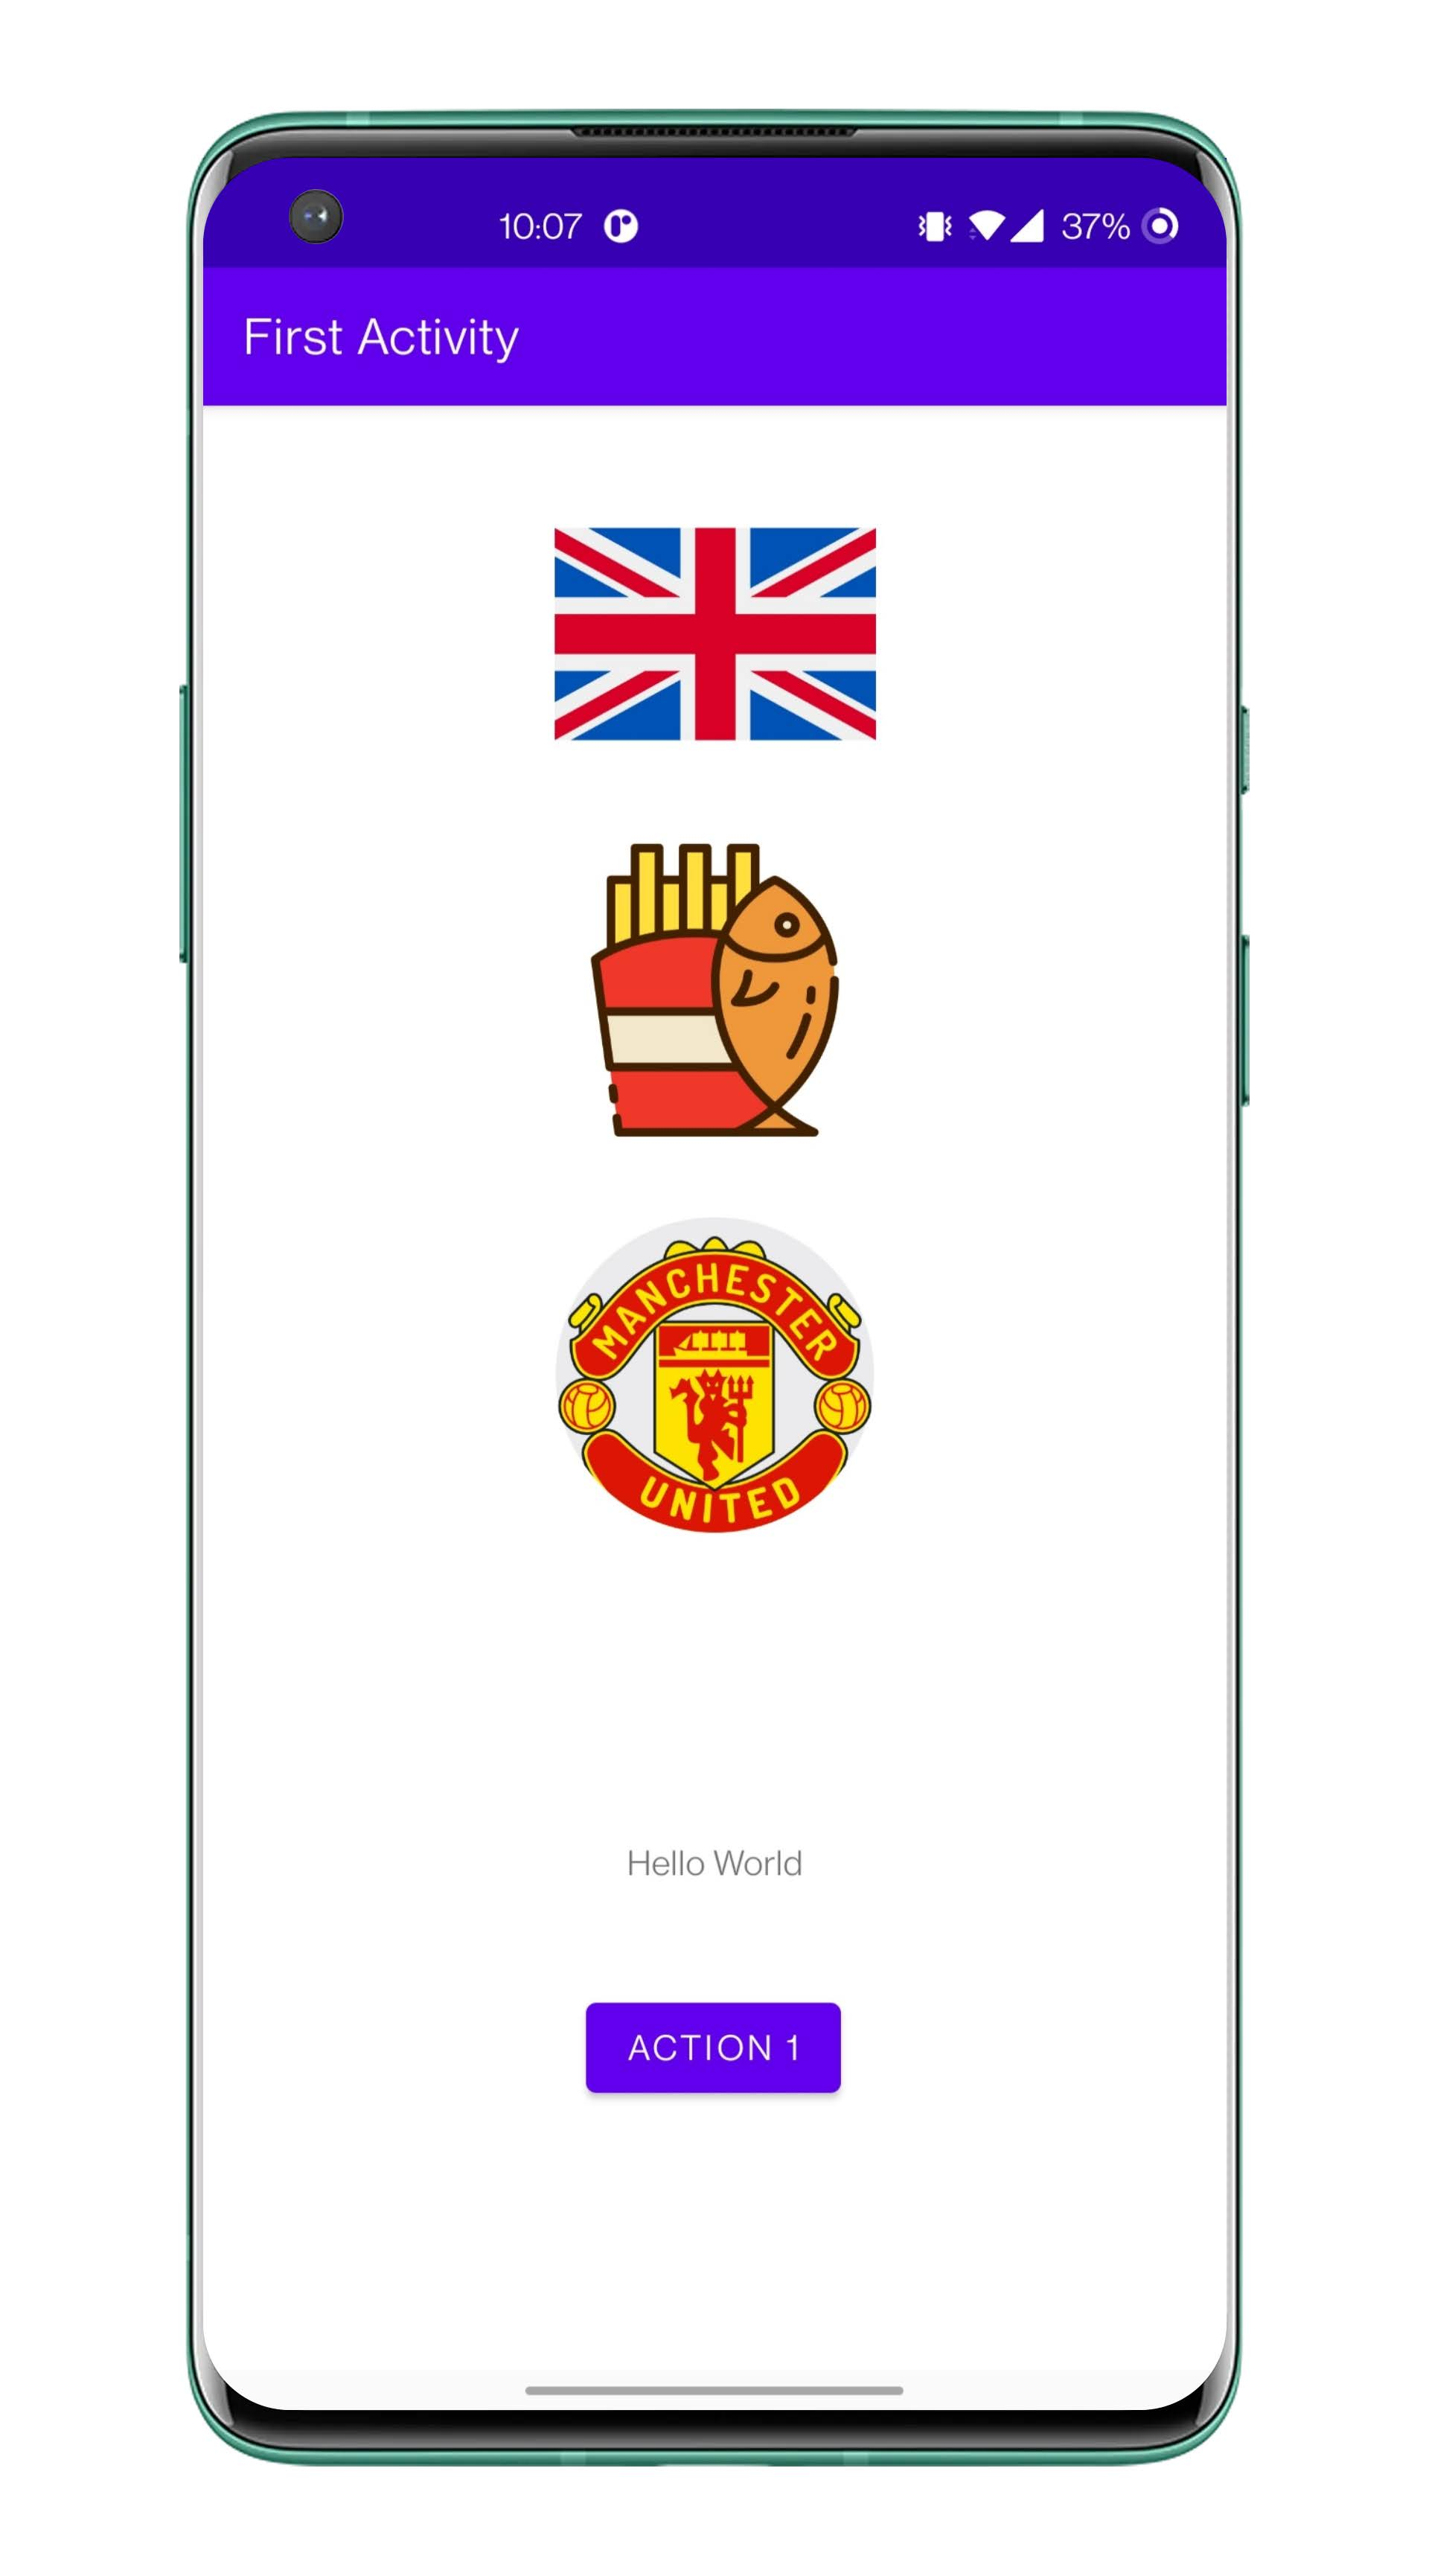
\includegraphics[scale = 0.12]{smartphone-vertical.jpg}
    \centering
    \caption{Aplicació en un mòbil, idioma anglès i orientació vertical}
    \label{vertical}
\end{figure}

\begin{figure}[!htbp]
    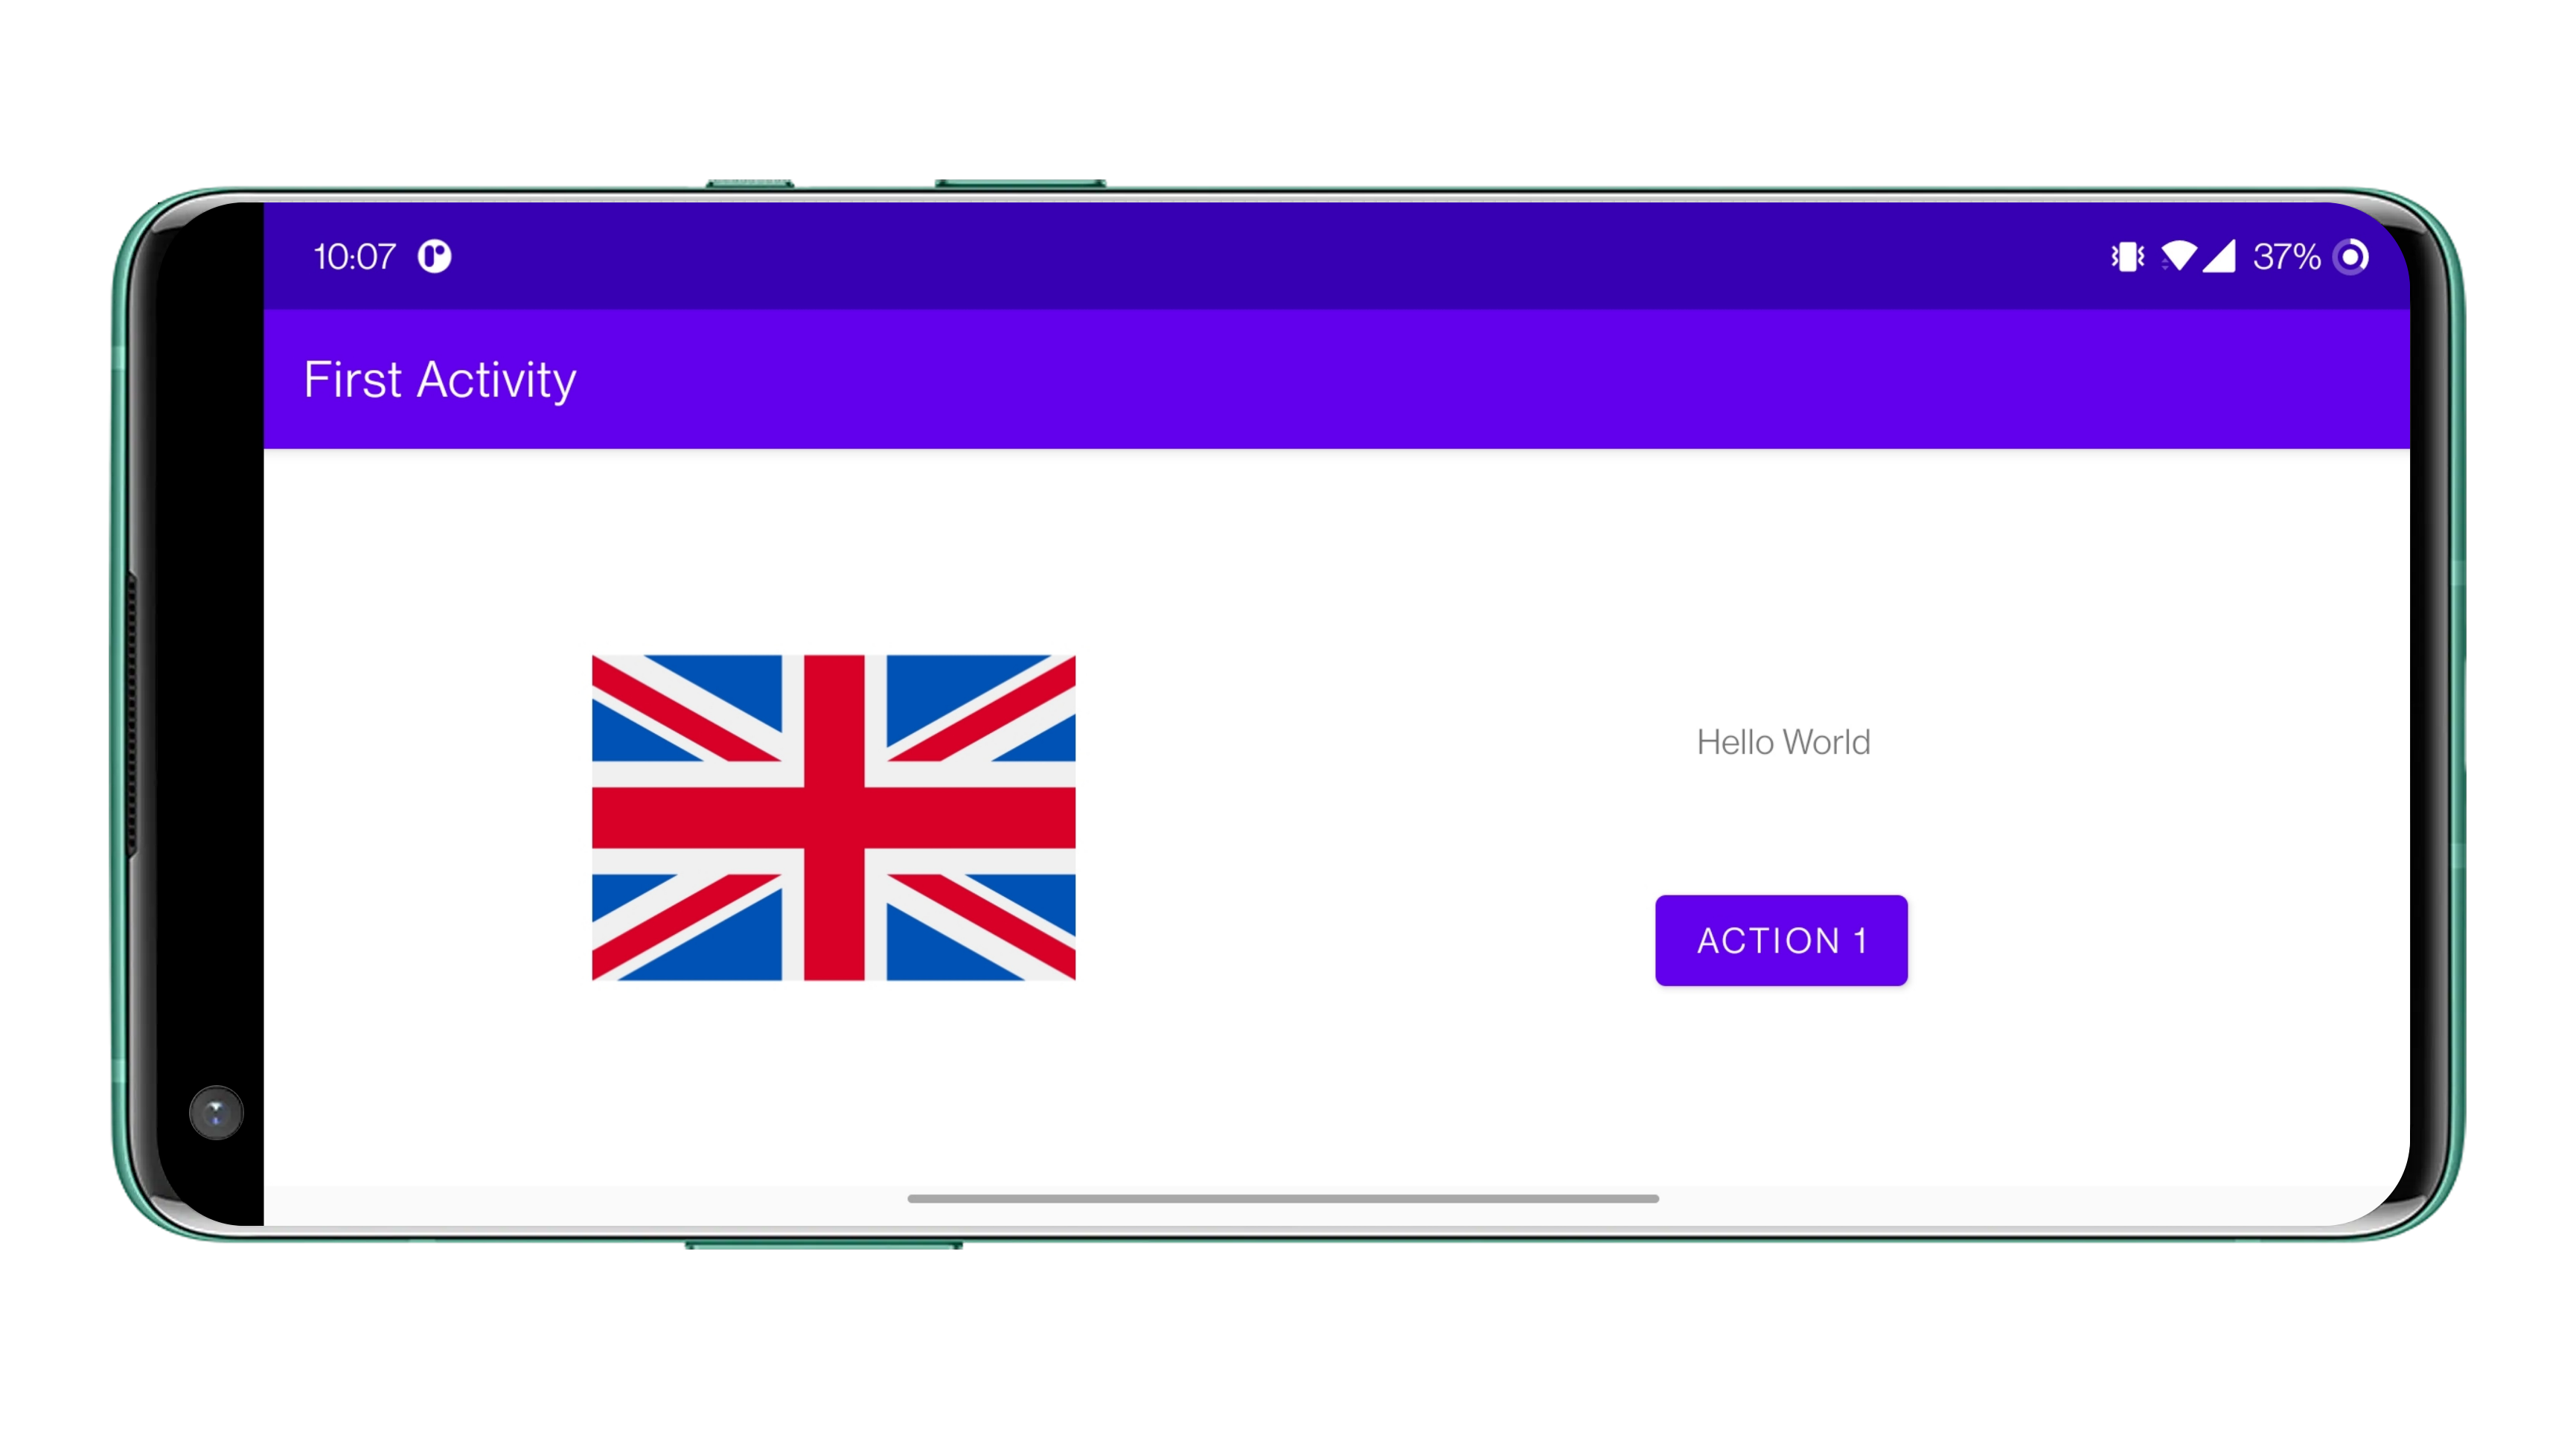
\includegraphics[scale = 0.12]{smartphone-land.PNG}
    \centering
    \caption{Aplicació en un mòbil, idioma anglès i orientació horitzontal}
    \label{vertical}
\end{figure}

\end{document}
